%File: formatting-instruction.tex
\documentclass[letterpaper]{article}
\usepackage{aaai}
\usepackage{times}
\usepackage{helvet}
\usepackage{courier}
\usepackage{hyperref}
\usepackage[round]{natbib}
\usepackage{graphicx}

\nocopyright
\frenchspacing
\pdfinfo{
/Title (Classification of Tweets by Company)
/Author (Curtis Ullerich, Daniel Stiner, Brandon Maxwell)}
\setcounter{secnumdepth}{0}  
\begin{document}

\title{Tweet Classification: Filtering \\ of Twitter for Company-relevant Tweets}
\author{
Curtis Ullerich, Daniel Stiner, Brandon Maxwell\\
Department of Computer Science and Engineering\\
Iowa State University
Ames, Iowa, USA\\
\{curtisu,stiner,bmaxwell\}@iastate.edu\\
}
\maketitle
\begin{abstract}
\begin{quote}
Twitter is a popular source for data mining due to its massive scale and inclusivity of current trends.
It is also a veritable goldmine of useful data for businesses seeking to discover public opinion about themselves or their products.
Using machine learning techniques, we analyze the accuracy of classifying whether tweets are part of the public opinion about a particular company or mearly contain keywords related to the company.
%Tweets present interesting classification challenges due to their irregular formatting and relatively small number of features.
%Classification purely by keyword filtering often suffers from a
%high accuracy and low recall, or low accuracy and high recall. % Q: Daniel - What does recall mean in this context? Also, list low accuracy first I think.
We aim to survey a variety of text processing steps combined with a Naive Bayes classifier, focusing on the effects of different tokenizations.
Our dataset consists of approximately 2,000 tweets of which 64\% are related to public opinion about the company Apple, Inc. The other 36\% are not, but still contain keywords related to the company.
Peliminary results have shown significant increases in accuracy % TODO insert actual numbers
by using domain-specific tokenizers, while suprisingly showing decreases in classification accurracy for other standard preproccessing methods such as n-grams.
\end{quote}
\end{abstract}

\section{Introduction}
Tweets are used as a source of data mining for applications ranging from predicting future stock price changes based on sentiment \citeauthor{Ruiz}, ... [ADD MORE]
In many cases, the problem of determining which tweets are relevant for a particular application is prerequisite to meaningful results. In some domains, filtering tweets based solely on keywords may be appropriate, but disambiguation remains an interest natural language processing problem in many cases. We present a system to disambiguate tweets about the company Apple.

\section{Related Work}
DUALIST is a system that extends Mallet by user-interactive feedback during training[Settles]. Included in their implementation was a TwitterPipe that performed some simple feature extraction. 
Part of the Sentiment Analysis Symposium focuses on tokenization of tweets for sentiment analysis, demonstrating that it provides consistent improvement over whitespace-based tokenizing \cite{potts2011}. A good deal of research has been done into sentiment classification of tweets, which requires very similar text processing and tokenization \cite{Pak10}. 

\section{Method}
\subsection{Corpus creation}
By accessing the Twitter \"Firehose\" stream through their public API, we harvested 115,000 tweets using broad keyword filters with the goal of collecting a superset of relevant tweets. This provides us a smaller set of features in the overall corpus. The keywords used for the company of choice during this round of testing, Apple, were collected manually from information on the company's website and the Wikipedia page about Apple:\\
...\\

This set of keywords clearly allows a large number of false positives:

\begin{table}[h]
\centering
\begin{tabular}{|l|}
	\hline
	nice fish and chip.. good pie apple :-) \\ http://t.co/KVDN5r5l \\ \hline
	20 chicken nuggets, chips, big mac, and a \\ vanilla milkshake LIFE IS GOOD \\ \hline
	1 more day whoop plus safari ride yay \\ \hline
	Ashley staples an apple.  "AHHHH!!!! \\ Apple juice in my eye!" \\ \hline
	I ain't seen uncle Mac in a while \\
	\hline
\end{tabular}
\caption{Examples of false positive tweets}
\label{tab:myfirsttable}
\end{table}


We define a tweet to be "about" Apple if the tweet mentions the company (via direct reference or stock symbol), one of its products, or a service it offers. We make the assumption that spam will be filtered from the testing set. This could be done via an existing Naive Bayes classifier, but we simply did not include instances of spam in our corpus during the manual labeling process. We collected our tweets over the course of twelve hours. On Twitter, a single message posted is often reposted, or "re-tweeted," many more times in a very short timespan. Because of the small timespan of our data collection, a large number of retweets (effectively duplicates) appeared in the dataset. We filtered these duplicates out of the dataset as well to prevent over-fitting in our model. After filtering, our original set of 115,000 tweets was reduced to 65,000. A representative sample of non-spam, non-duplicate tweets has composition of 60\% topical instances and 40\% false positives [need to analyze this for sure].

A computer-posted spam tweet:
\begin{table}[h]
\centering
\begin{tabular}{|l|}
	\hline
	I've collected 10,650 gold coins! \\ http://t.co/H0V0O6yP \#ipad, \#ipadgames, \#gameinsight\\
	\hline
\end{tabular}
\end{table}


A retweet, signified by "RT":
\begin{table}[h]
\centering
\begin{tabular}{|l|}
	\hline
	RT @PHILerNotebook: Trying to fix my Mac. \\ This gray loading bar takes 10 minutes to start up. \\ Grr. Shall take it to an \_Apple\_ \_store\_ soon! \\
	\hline
\end{tabular}
\end{table}

We hand labeled 2000 tweets for use in training and testing, including only English-language tweets in our training set. \\
Data sets and scripts used for processing text data are available on the project website. (http://tweets.curtisullerich.com/)\\

\subsection{Preprocessing Pipeline}

We do all machine learning with the Mallet library developed by the University of Massachusetts \cite{McCallumMALLET}. Mallet includes abstractions for a data processing pipeline, during which we use both existing and custom processing "Pipes" to transform the data, beginning in our case with raw tweets text and ending in Mallet's internal FeatureVector format. We built several Pipes to analyze the effect of different filters and processes on the accuracy of classification. Not every Pipe proved to increase accuracy--some decreased it. We present the descriptions of and motivations for these Pipes here.

\subsubsection{Feature-space Enrichment} ~\\
\textit{Stopword removal}: We wrote a Pipe to remove any tokens that appeared in a list of the 50 most common words in the English language.\\
~\\
\textit{N-grams}: Using n-grams is a common method of increasing the number of features present in short text [FIND CITATION]. Often, this is enough to increase accuracy significantly. During our testing, this was not the case. Rather, including bigrams and trigrams actually reduced accuracy slightly.\\
~\\
\textit{HTML corrections}: When accessing tweets through Twitter's public API, the native JSON format includes HTML-encoded entities that can add confusing features to the tweets if not un-escaped. For instance, angle brackets are replaced with \&lt; and \&gt; (less-than and greater-than), causing emoticons, for instance, to no longer be parseable. The emoticon \">.<", for instance, would be "\&gt;.\&lt;". This Pipe un-escapes all such entities, making them easier to parse.\\
~\\
\textit{URL replacement}: 
~\\
\textit{Spell checking}: Twitter's user-generated content contains a large volume of misspelled words. Using a spell-checking library, we wrote a Pipe to replace unrecognized words (misspelled words) with their corrections if the confidence for correction was above a certain threshold. \\
~\\
\subsubsection{Disambiguation}
~\\
\textit{Stemming}: Stemming is the process of reducing words to their "stem." While this stem does not necessarily have to be the root of the word, it should satisfy the property that related words have the same stem. Therefore the stem of the related words "argue," "argued," and "arguing" all have the stem of "argu," even though argu is not the true linguistic stem. We used the standard Porter stemmer to implement this[CITATION].\\

\begin{figure*}[t!]
\centering
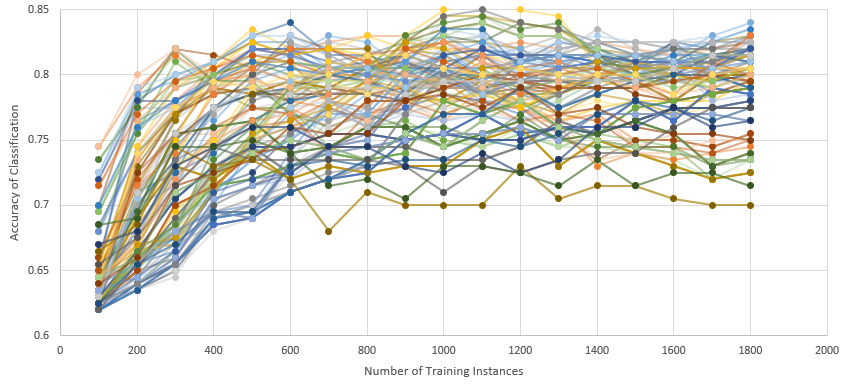
\includegraphics[height=7cm]{chart}
\caption{Accuracy Chart}
\label{fig:chart}
\end{figure*}

\subsubsection{Tokenization}
~\\
Twitter data, and user-generated web content in general, provides unique challenges to an automatic tokenization system due to the high level of noise in the feature set [citation and more details]. Tweets are limited to 140 characters, which limits the total number of features possible. Some of the many natural language processing dilemmas present in tweets include excessive and irregular punctuation, frequent misspellings, emoticons, URLs, and hashtags, to name a few.\\

\begin{table}[h]
\centering
\begin{tabular}{|l|}
	\hline
	Cool ranch , 4 berry sundae , apple juice \#yessuh \\ \#latenight \#snack http://t.co/ttc3vujp \\ \hline
	I just poured apple juice on my cereal.. Gah. \#SoTired \\ \hline
	I hate Siri.. -\_\_\_- \\
	\hline
\end{tabular}
\caption{Examples of difficult tokenizations}
\label{tab:tokenization_examples}
\end{table}

We approach this problem using a layered token extraction system. Using regular expressions, we begin by searching for tokens that may include other, more general tokens. A prime example of this is an emoticon appearing in a URL.

Searching for emoticons in this tweet will extract :/ as an emoticon, effectively breaking up the URL.
\begin{quote}
\textit{Now on my iphone ?? http://t.co/Rqr1RL2R}
\end{quote}

Additionally, users often include emoticons or links after text with no delimiting whitespace. 

\begin{quote}
\textit{I listen to my iPod every day and it's just broke omg:(!!}
\end{quote}

Extracting tokens using this layered approach eliminates many of these problems.

After tokenizing these special features in order (URLs, emoticons, usernames, and hashtags) we are left with a fragmented tweet containing myriad punctuation, capitalization, and creative spellings. As done by \citet{potts2011} we normalize the length of all letter sequences greater than two, as in English, these are invariably due to user-added emphasis, and condensing the larger set of tokens focuses the feature set. In the following tweet, "loooool" is normalized to "loool".
\begin{quote}
\#news can't wait for my signed \#OoRITE2OutNow it's emotional here right now loooool \#OoRITE2OutNow https://t.co/r4n4cn6C 
\end{quote}

Note that such repetitions are often valid in URLs and some emoticons. Normalizing them prior to this step would make URLs invalid if using our link replacement Pipe.

As presented in our results, because of irregular capitalization, two tokens likely to be semantically identical with respect to company classification may be represented in multiple cases: {Nooo, NOOO, nooo, NoOo} is a prime example. To alleviate this, we attempt three different approaches. In the first, we simply lowercase all remaining tokens (note that many URLs become invalid after modifying case). In the second, we lowercase any text that is not in all caps. This serves to retain acronyms. In the third, we change all remaining tokens to lowercase, leaving the case of all strings containing "apple" (case insensitive) alone. We made this decision based on the semantic difference between the capitalization of Apple the company and apple the fruit. While correct capitalization is naturally not always present for this token, this is one case where capitalization serves to disambiguate. This same principle can be generalized to a larger set of keywords and applied to other companies in a similar fashion. 

\section{Experimental Setup}
...constant-size test set with sliced training
...comparison to n-fold validation

Lorem ipsum dolor sit amet, consectetur adipiscing elit. Maecenas vulputate ultricies lorem, quis consectetur erat tristique id. Nulla eget nunc in urna vestibulum ornare ac sed purus. Curabitur consequat gravida turpis in rutrum. Nulla vehicula condimentum luctus. Nam venenatis facilisis orci sed ullamcorper. In felis leo, rutrum nec vestibulum vitae, lacinia at ipsum. Praesent orci nibh, pellentesque vitae placerat eget, tempus eget libero. Duis eleifend, orci nec pretium condimentum, quam erat euismod quam, sed accumsan erat lacus in felis. Aliquam vitae leo sem. Cum sociis natoque penatibus et magnis dis parturient montes, nascetur ridiculus mus. Etiam consequat ante eu turpis molestie vel gravida felis varius. Vestibulum tincidunt, velit quis convallis imperdiet, est nisi aliquet mauris, eget tempus metus eros eget erat. Aenean sit amet dui vel urna pretium dictum nec sed elit. Vivamus feugiat dictum neque imperdiet ultrices. Nullam commodo rhoncus elit id adipiscing. Nam nec turpis ut nisi pulvinar blandit at tincidunt dolor.

Integer dictum tristique felis vitae lobortis. Quisque hendrerit, mi vel vestibulum sagittis, nulla leo rhoncus nisl, ac lobortis nisi lorem quis nisl. Nullam vehicula magna convallis odio semper vestibulum. Ut lobortis, purus eu sodales congue, sapien dolor consectetur turpis, vitae luctus nibh elit et eros. Nam tempor felis eget dui laoreet vehicula. Praesent imperdiet hendrerit elit sed tempus. Phasellus feugiat pretium metus id scelerisque. Morbi ligula lectus, blandit in vestibulum id, fermentum sit amet augue. Donec pharetra molestie euismod. Nulla porttitor feugiat purus, in egestas lorem venenatis sed. Phasellus quis interdum diam. Ut congue, magna at malesuada luctus, augue urna dignissim nulla, congue lacinia metus felis eget odio. Vestibulum et nisl sodales quam commodo laoreet. Ut a tortor tortor.

\section{Results}

...baseline using priors
  baseline using whitespace splitting in naive bayes.
  select interesting improvements.
  graphs of both validation types
  most useful features for classification

Lorem ipsum dolor sit amet, consectetur adipiscing elit. Maecenas vulputate ultricies lorem, quis consectetur erat tristique id. Nulla eget nunc in urna vestibulum ornare ac sed purus. Curabitur consequat gravida turpis in rutrum. Nulla vehicula condimentum luctus. Nam venenatis facilisis orci sed ullamcorper. In felis leo, rutrum nec vestibulum vitae, lacinia at ipsum. Praesent orci nibh, pellentesque vitae placerat eget, tempus eget libero. Duis eleifend, orci nec pretium condimentum, quam erat euismod quam, sed accumsan erat lacus in felis. Aliquam vitae leo sem. Cum sociis natoque penatibus et magnis dis parturient montes, nascetur ridiculus mus. Etiam consequat ante eu turpis molestie vel gravida felis varius. Vestibulum tincidunt, velit quis convallis imperdiet, est nisi aliquet mauris, eget tempus metus eros eget erat. Aenean sit amet dui vel urna pretium dictum nec sed elit. Vivamus feugiat dictum neque imperdiet ultrices. Nullam commodo rhoncus elit id adipiscing. Nam nec turpis ut nisi pulvinar blandit at tincidunt dolor.

Integer dictum tristique felis vitae lobortis. Quisque hendrerit, mi vel vestibulum sagittis, nulla leo rhoncus nisl, ac lobortis nisi lorem quis nisl. Nullam vehicula magna convallis odio semper vestibulum. Ut lobortis, purus eu sodales congue, sapien dolor consectetur turpis, vitae luctus nibh elit et eros. Nam tempor felis eget dui laoreet vehicula. Praesent imperdiet hendrerit elit sed tempus. Phasellus feugiat pretium metus id scelerisque. Morbi ligula lectus, blandit in vestibulum id, fermentum sit amet augue. Donec pharetra molestie euismod. Nulla porttitor feugiat purus, in egestas lorem venenatis sed. Phasellus quis interdum diam. Ut congue, magna at malesuada luctus, augue urna dignissim nulla, congue lacinia metus felis eget odio. Vestibulum et nisl sodales quam commodo laoreet. Ut a tortor tortor.

Phasellus et mi eu est fermentum cursus id sodales nisi. Maecenas sodales ornare mauris, nec cursus mi commodo non. In pulvinar odio id est pharetra cursus. Fusce blandit scelerisque bibendum. Aliquam erat volutpat. Aliquam tellus lorem, pharetra a vehicula nec, tincidunt sit amet felis. Nullam nec sapien quis leo facilisis commodo at vel enim. Suspendisse ultricies massa at nisl iaculis scelerisque. Phasellus sed sodales augue. Pellentesque a nisl enim.

Mauris at eros velit, non venenatis augue. Fusce vel ornare purus. Praesent condimentum lectus sit amet sem ullamcorper eget euismod tellus dapibus. Aenean fringilla urna vel nisl accumsan imperdiet. Duis cursus mattis molestie. Phasellus est lorem, condimentum quis congue eget, condimentum scelerisque arcu. Phasellus odio lacus, imperdiet at convallis et, vehicula a nisi. Mauris consequat urna vitae ipsum vulputate ullamcorper. Fusce ullamcorper mauris dolor. Quisque gravida hendrerit tristique. Fusce magna urna, vestibulum eget condimentum eu, semper sit amet felis. Ut placerat hendrerit neque id vestibulum. Phasellus convallis, nulla at fermentum bibendum, massa risus tempus eros, et malesuada diam enim sed purus. Praesent tincidunt dapibus lobortis. Curabitur sodales dignissim est quis tempus.

Aenean vel enim eu mauris scelerisque pulvinar in quis odio. Suspendisse eu sapien vitae eros ultrices congue volutpat quis elit. Aliquam nisl nibh, hendrerit ut feugiat eget, gravida eget urna. In nisl felis, elementum ut sollicitudin non, fringilla in neque. Aliquam quis luctus lacus. Cras et mauris sem, vel imperdiet sapien. Suspendisse in ligula id turpis adipiscing sodales vitae ut lectus. Vestibulum neque nulla, commodo vitae venenatis id, accumsan vitae odio. Quisque velit purus, tempor non porta laoreet, elementum vel sem. Nullam mollis euismod dolor, eget pulvinar elit cursus eget. Nunc quis pharetra odio. Donec lacus leo, pulvinar quis vestibulum eget, porta id nibh.


\section{Conclusion and Future Work}

We could test the robustness of this system by applying this process to other companies for a similar-length time slice of training data. We could also test this model against tweets from a different time span to determine whether the data is subject to temporal overfitting, and to what degree.

[These guys] demonstrate a system of using background knowledge and relatedness, in which current information in the Twitter stream is used to more accurately estimate the priors for a Naive Bayes classification.

Inclusion of background knowledge.

Use of Wikipedia for disambiguation.


Lorem ipsum dolor sit amet, consectetur adipiscing elit. Maecenas vulputate ultricies lorem, quis consectetur erat tristique id. Nulla eget nunc in urna vestibulum ornare ac sed purus. Curabitur consequat gravida turpis in rutrum. Nulla vehicula condimentum luctus. Nam venenatis facilisis orci sed ullamcorper. In felis leo, rutrum nec vestibulum vitae, lacinia at ipsum. Praesent orci nibh, pellentesque vitae placerat eget, tempus eget libero. Duis eleifend, orci nec pretium condimentum, quam erat euismod quam, sed accumsan erat lacus in felis. Aliquam vitae leo sem. Cum sociis natoque penatibus et magnis dis parturient montes, nascetur ridiculus mus. Etiam consequat ante eu turpis molestie vel gravida felis varius. Vestibulum tincidunt, velit quis convallis imperdiet, est nisi aliquet mauris, eget tempus metus eros eget erat. Aenean sit amet dui vel urna pretium dictum nec sed elit. Vivamus feugiat dictum neque imperdiet ultrices. Nullam commodo rhoncus elit id adipiscing. Nam nec turpis ut nisi pulvinar blandit at tincidunt dolor.

Integer dictum tristique felis vitae lobortis. Quisque hendrerit, mi vel vestibulum sagittis, nulla leo rhoncus nisl, ac lobortis nisi lorem quis nisl. Nullam vehicula magna convallis odio semper vestibulum. Ut lobortis, purus eu sodales congue, sapien dolor consectetur turpis, vitae luctus nibh elit et eros. Nam tempor felis eget dui laoreet vehicula. Praesent imperdiet hendrerit elit sed tempus. Phasellus feugiat pretium metus id scelerisque. Morbi ligula lectus, blandit in vestibulum id, fermentum sit amet augue. Donec pharetra molestie euismod. Nulla porttitor feugiat purus, in egestas lorem venenatis sed. Phasellus quis interdum diam. Ut congue, magna at malesuada luctus, augue urna dignissim nulla, congue lacinia metus felis eget odio. Vestibulum et nisl sodales quam commodo laoreet. Ut a tortor tortor.


\section{Contributions}
We have built several reusable Java components that extend the Mallet API for processing of data from Twitter. We created a TweetJsonIterator that accepts a file of Twitter's JSON-formatted tweets and creates training Instances containing their values for easy processing during model training. We have implemented several Pipes that can be reused or easily modified to suit a similar Twitter processing purpose. These include Link2Title, Stemmer, SpellCheck, and Tokenize, the latter of which serves as a more extensible tokenizer than Mallet's default. All code is available through our project website. We also provide a corpus of 115,000 tweets selected by Apple-related keyword and our labeled data set of 2000 tweets. The bash scripts used to filter the data for near-duplicates and spam are also available for download.

\section{ Acknowledgments}
Thank you to Dr. Jin Tian and our class teaching assistant, Ru He, for their helpful guidance during this research project. We also extend our thanks to our friends for their help in manual labeling of tweets.


\bibliographystyle{plainnat}
\bibliography{paper}

%[1] J. Bollen, H. Mao, and X.-J. Zeng. Twitter mood predicts the stock market. Journal of Computational Science, abs/1010.3003, 2010\\

\end{document}
